\documentclass[10pt]{article}

\usepackage[margin=1in]{geometry}
% https://tex.stackexchange.com/questions/27802/set-noindent-for-entire-file
\setlength\parindent{0pt}
% https://tex.stackexchange.com/questions/9550/why-does-underlined-text-not-get-wrapped-once-it-hits-the-end-of-a-line
\usepackage{soul}
\usepackage{indentfirst}
\usepackage{amsmath,amsthm,amssymb,scrextend}
\DeclareMathOperator*{\argmax}{arg\,max}
\DeclareMathOperator*{\argmin}{arg\,min}
% \usepackage{fancyhdr}
% \setlength{\headheight}{14.49998pt}
% \pagestyle{fancy}
\usepackage{graphicx}

\newcommand{\cont}{\subseteq}
\usepackage{tikz}
\usepackage{pgfplots}
\pgfplotsset{width=10cm,compat=1.9}

\usepackage{amsmath}
\usepackage[mathscr]{euscript}
\let\euscr\mathscr \let\mathscr\relax
\usepackage[scr]{rsfso}
\usepackage{amsthm}
\usepackage{amssymb}
\usepackage{multicol}

\usepackage{algorithm}
\usepackage{algpseudocode}

\usepackage{listings}
\usepackage{xcolor}
\usepackage{float}
\definecolor{codegreen}{rgb}{0,0.6,0}
\definecolor{codegray}{rgb}{0.5,0.5,0.5}
\definecolor{codepurple}{rgb}{0.58,0,0.82}
\definecolor{backcolour}{rgb}{0.95,0.95,0.92}

\lstdefinestyle{mystyle}{
    backgroundcolor=\color{backcolour},   
    commentstyle=\color{codegreen},
    keywordstyle=\color{magenta},
    numberstyle=\tiny\color{codegray},
    stringstyle=\color{codepurple},
    basicstyle=\ttfamily\footnotesize,
    breakatwhitespace=false,         
    breaklines=true,                 
    captionpos=b,                    
    keepspaces=true,                 
    numbers=left,                    
    numbersep=5pt,                  
    showspaces=false,                
    showstringspaces=false,
    showtabs=false,                  
    tabsize=2
}

\lstset{style=mystyle}

\DeclareMathOperator{\arcsec}{arcsec}
\DeclareMathOperator{\arccot}{arccot}
\DeclareMathOperator{\arccsc}{arccsc}
\newcommand{\ddx}{\frac{d}{dx}}
\newcommand{\dfdx}{\frac{df}{dx}}
\newcommand{\ddxp}[1]{\frac{d}{dx}\left( #1 \right)}
\newcommand{\dydx}{\frac{dy}{dx}}
\let\ds\displaystyle
\newcommand{\intx}[1]{\int #1 \, dx}
\newcommand{\intt}[1]{\int #1 \, dt}
\newcommand{\defint}[3]{\int_{#1}^{#2} #3 \, dx}
\newcommand{\imp}{\Rightarrow}
\newcommand{\un}{\cup}
\newcommand{\inter}{\cap}
\newcommand{\ps}{\mathscr{P}}
\newcommand{\set}[1]{\left\{ #1 \right\}}
\newtheorem*{sol}{Solution}
\newtheorem*{claim}{Claim}
\newtheorem{problem}{Problem}
\def\mathbi#1{\textbf{\em #1}}
\begin{document}

% \lhead{Stats 303}
% \chead{Luyao Wang lw337}
% \rhead{\today}

\begin{center}
  {\Large \bf COMPSCI 308: Design and Analysis of Algorithms Homework 2}
  \vspace{2mm}

  {\bf Luyao Wang}

  {\today}
\end{center}

\section*{1. Divide and Conquer}
\subsection*{(a) Programming}

\begin{enumerate}
  \item {Iterative Fibonacci number computation

        \begin{verbatim}
def fibonacci_iterative(n: int) -> int:
    if n < 0:
        raise Exception("n should be larger than or equal to 0")
    elif n == 0:
        return 0
    elif n == 1:
        return 1

    fib_minus_2 = 0
    fib_minus_1 = 1
    fib = 0

    for i in range(3, n + 1):
        fib = fib_minus_2 + fib_minus_1
        fib_minus_2 = fib_minus_1
        fib_minus_1 = fib

    return fib
            \end{verbatim}

        The time complexity is $O(n)$ because we use one for loop with $i$ from $3$ to $n$, inside the for loop, each execution is constant time.


        \begin{figure}[H]
          \centering
          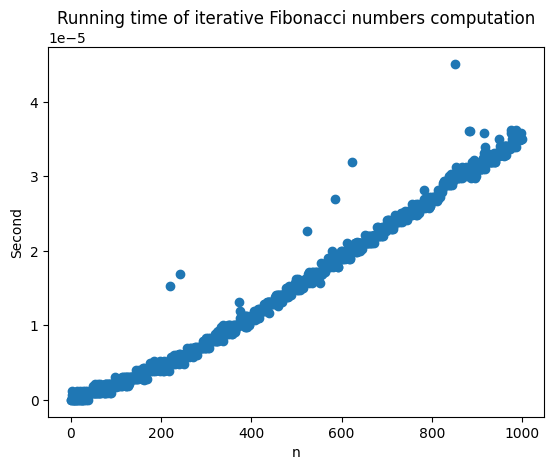
\includegraphics[width=0.8\textwidth]{../assets/runtimes_iterative.png}
          \caption{Running time of iterative Fibonacci numbers computation}
        \end{figure}
        }
  \item {Recursive Fibonacci number computation
        \begin{verbatim}
def fibonacci_recursive(n: int) -> int:
    if n < 0:
        raise Exception("n should be larger than or equal to 0")
    elif n == 0:
        return 0
    elif n == 1:
        return 1
    else:
        return fibonacci_recursive(n - 1) + fibonacci_recursive(n - 2)
            \end{verbatim}



        The time of computing Fibonacci recursively is $T(n) = T(n-1) + T(n-2) + O(1)$.

        Fibonacci can be mathematically represented as a linear recursive function $F(n) = F(n-1) + F(n-2)$.

        The characteristic equation for this function will be $x^2 = x + 1$.
        Solving this by quadratic formula we can get the roots as $x = \frac{1+\sqrt{5}}{2}$ and $x = \frac{1-\sqrt{5}}{2}$.

        For the Fibonacci function $F(n) = F(n-1) + F(n-2)$ the solution will be:

        \begin{align*}
          F(n) = \left( \frac{1+\sqrt{5}}{2} \right)^n + \left( \frac{1-\sqrt{5}}{2} \right)^n
        \end{align*}

        $T(n)$ and $F(n)$ are asymptotically the same as both functions are representing the same thing.

        \begin{align*}
          T(n) = O \left( \left( \frac{1+\sqrt{5}}{2} \right)^n + \left( \frac{1-\sqrt{5}}{2} \right)^n \right)
        \end{align*}

        \begin{align*}
          T(n) = O \left( \left( \frac{1+\sqrt{5}}{2} \right)^n \right) \
        \end{align*}

        From the experiment results in the table, we can see that the ratio between two consecutive $n$s is close to $\frac{1+\sqrt{5}}{2}$, or the golden ratio.

        \begin{table}[H]
          \centering
          \caption{Running time for different $n$}
          \label{tab:csv_data}
          \begin{tabular}{cc}
            \hline
            \textbf{$n$} & \textbf{seconds} \\
            \hline
            35           & 1.12             \\
            36           & 1.82             \\
            37           & 2.95             \\
            38           & 4.78             \\
            39           & 7.76             \\
            40           & 12.56            \\
            \hline
          \end{tabular}
        \end{table}

        \begin{figure}[H]
          \centering
          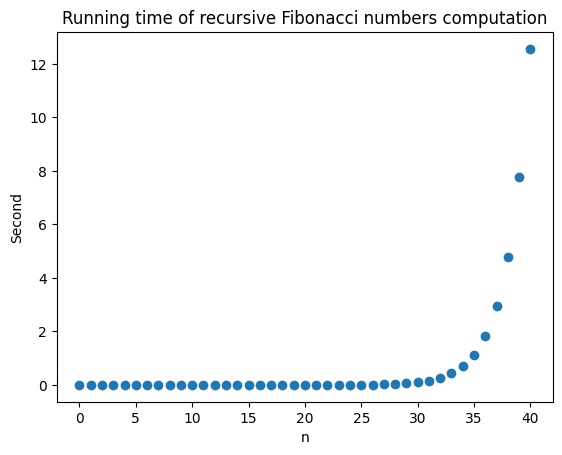
\includegraphics[width=0.8\textwidth]{../assets/runtimes_recursive.png}
          \caption{Running time of recursive Fibonacci numbers computation}
        \end{figure}
        }
\end{enumerate}

\subsection*{(b) Recursion Tree}

Recurrence equation representing the algorithm:

\[T(n) = 5T(\frac{n}{2}) + n\]

\begin{figure}[H]
  \centering
  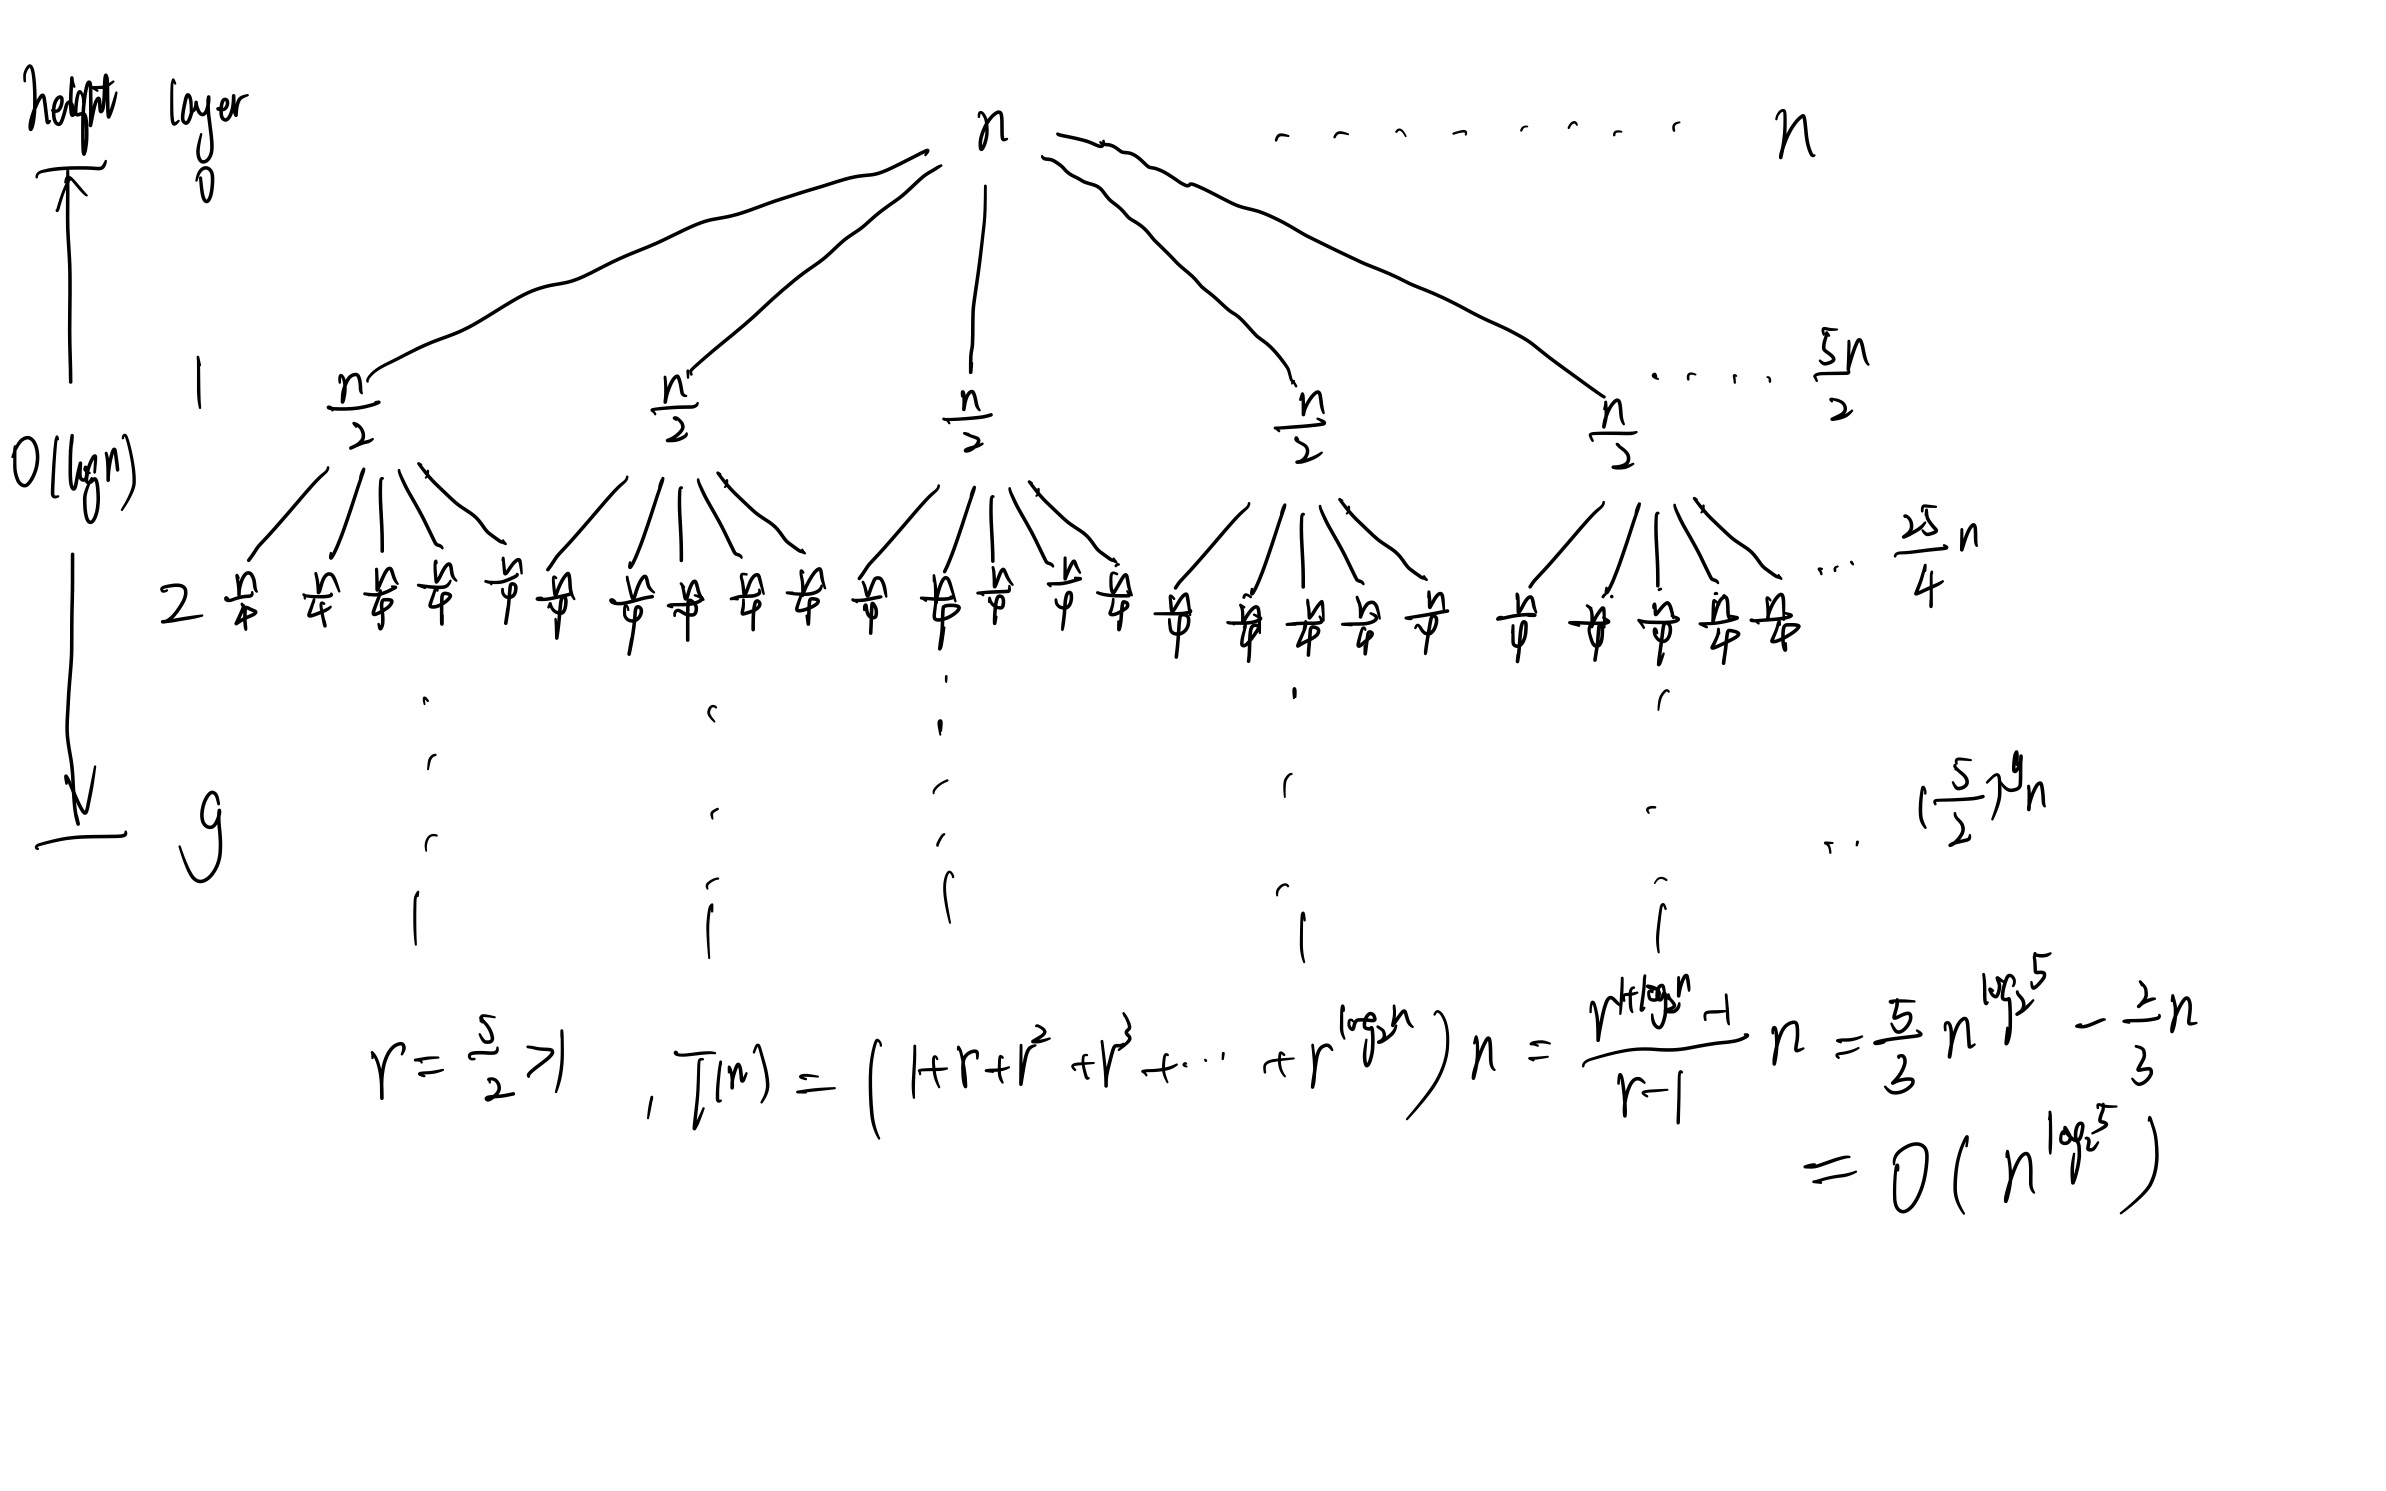
\includegraphics[width=\linewidth]{../assets/1_b.png}
\end{figure}

\subsection*{(c) Asymptotic Analysis}

\begin{enumerate}

  \item{First algorithm

        \[T(n) = 4T(n-1) + 1\]

        Solve by subtituiton:

        \begin{align*}T(n) & =  4T(n-1) + 1                         \\
                   & = 4(4T(n-2)+1) + 1                     \\
                   & = 4 \cdot 4T(n-2) + 1 + 4              \\
                   & = 4 \cdot 4(4T(n-3)+1) + 1 + 4         \\
                   & = 4 \cdot 4 \cdot 4T(n-3) + 1 + 4 + 16 \\
                   & = \cdots                               \\
                   & = 4^iT(n-i) + \sum_{t=0}^{i-1}4^t      \\
                   & = 4^iT(n-i) + \frac{4^i-1}{3}
        \end{align*}

        Base case $i=n-1$, $T(1)=1$.

        Therefore,
        \begin{align*}T(n) & =  4^iT(n-i) + \frac{4^i-1}{3}  \\
                   & = 4^{n-1} + \frac{4^{n-1}-1}{3} \\
                   & = \frac{4^{n}-1}{3}             \\
                   & = \Theta(n^4)
        \end{align*}
        }

  \item{Second algorithm

        \[T(n) = 3T(\frac{n}{3}) + n^5\]

        By Master Theorem, $a=3$, $b=3$, $n^{\log _b a}=n$ is polynomially smaller than $n5$.

        Therefore, case 3 of Master Theorem fits, $T(n) = \Theta(n^5)$
        }

  \item {Conclusion

        Considering the asymptotic behaviors of the two algorithms, the first is preferable.
        }
\end{enumerate}



\section*{2. Dynamic Programming}

\subsection*{(a) Pseudocode}

\begin{algorithm}[H]
  \caption{Dynamic Programming Algorithm for Maximum Success Score}
  \begin{algorithmic}[1]
    \Function{MaxSuccessScore}{$i, j, \text{memo}$}
    \If{$\text{memo}[i][j]$ is defined}
    \State \Return $\text{memo}[i][j]$
    \EndIf

    \State $\text{maxScore} \gets 0$

    \For{$k = i \text{ to } j$}
    \State $\text{score} \gets \text{cheatIndex}[k]$

    \If{$k > i$}
    \State $\text{score} \times= \text{cheatIndex}[k-1]$
    \EndIf
    \If{$k < j$}
    \State $\text{score} \times= \text{cheatIndex}[k+1]$
    \EndIf

    \If{$k > i$}
    \State $\text{score} += \text{MaxSuccessScore}(i, k-1, \text{memo})$
    \EndIf
    \If{$k < j$}
    \State $\text{score} += \text{MaxSuccessScore}(k+1, j, \text{memo})$
    \EndIf

    \State $\text{maxScore} \gets \max(\text{maxScore}, \text{score})$
    \EndFor

    \State $\text{memo}[i][j] \gets \text{maxScore}$
    \State \Return $\text{maxScore}$
    \EndFunction

    \Function{CalculateMaxSuccessScore}{$\text{cheatIndex}$}
    \State $n \gets \text{length}(\text{cheatIndex})$
    \State $\text{memo} \gets \text{new DiagonalMatrix}(n, n)$
    \State \Return \Call{MaxSuccessScore}{1, n, \text{memo}}
    \EndFunction
  \end{algorithmic}
\end{algorithm}

\subsection*{(b) Asymptotic Analysis}

In this algorithm, the number of subproblems is determined by the range of indices $i$ and $j$. Since each subproblem corresponds to a specific range, there are a total of $O(n^2)$ possible subproblems, where $n$ is the length of the \texttt{cheatIndex} array.

For each subproblem, the algorithm performs a loop from $i$ to $j$, resulting in a linear time complexity of $O(n)$ for each subproblem. Within this loop, the algorithm performs constant-time operations such as multiplication, addition, and memoization.

More formally,

\begin{align*}T(n) & =  \sum_{k=1}^{n}(n+1-k)k                            \\
                   & =  \sum_{k=1}^{n}(n+1)k - k^2                        \\
                   & =  n\frac{n+1 + n^2 + n}{2} - \frac{n(n+1)(2n+1)}{6} \\
                   & = \frac{n^3 + 3n^2 + 2n}{6}
\end{align*}


Therefore, the overall time complexity of the algorithm is $O(n^3)$.

\end{document}